\section{The first fundamental form}
Now we do some geometry. 
\subsection{Lengths of curves on surfaces}
\begin{definition}[]
    Let $p \in S$. The \textbf{first fundamental form} of $S$ at $p$ associates to tangent vectors $v,w \in T_pS$ the scalar $\langle v,w \rangle _{p,S}=v\cdot w.$
\end{definition}
This is an inner product for $S$ at $p$. If you know how tensors work, at each point we can write $g=g^{(x)}_{ij}dx^i \otimes dx^j $, and we can calculate the coefficients of the metric tensor by $g_{ij}=g(\partial _i ,\partial _j )_x=\langle \partial _i ,\partial _j  \rangle _x$. Traditionally, for $\sigma(u,v)$ a patch, if $p \in \im \sigma$ we have $\partial _u\sigma,\partial _v\sigma$ spanning $T_pS$. Define $du \colon T_pS \to \R,\ dv \colon T_p S \to \R$, by \[
    du(v)=\lambda,\quad dv(v)=\mu \quad \text{if} \ v=\lambda \partial _u\sigma +\mu \partial _v\sigma.
\] (These are $1$-forms, the basis vectors of the cotangent space.) Then $\langle v,v \rangle =\lambda ^2\langle \partial _u\sigma,\partial _u\sigma \rangle +2\lambda \mu \langle \partial _u\sigma,\partial _v\sigma \rangle +\mu^2\langle \partial _v\sigma,\partial _v\sigma \rangle $. If we write $E=\|\partial _u\sigma\|^2,\ F=\partial _u\sigma \cdot \partial _v\sigma,\ G=\|\partial _v\sigma\|^2$, then \[
\langle v,v \rangle =E\lambda^2+2F\lambda \mu+G\mu^2=Edu^2+2Fdudv+Gdv^2.
\] If $\gamma \subseteq \im \sigma$, $\gamma (t)=\sigma(u(t),v(t))$ for $u,v$ smooth. Then $\dot \gamma =\dot u\partial _u\sigma+\dot v\partial _v\sigma$, so $\langle \dot \gamma ,\dot \gamma  \rangle =E\dot u^2+2F\dot u\dot v+G\dot v^2$, and the length of $\gamma $ is given by $\int (E\dot u^2+2F\dot u\dot v+G\dot v^2)^{1 /2} \, dt$.

\begin{example}
    For a plane $\sigma(u,v)=\mathbf a+u\mathbf p+v\mathbf q$ for unit vectors $\mathbf p\perp \mathbf q$, we have $\partial_u\sigma =\mathbf p, \partial _v\sigma=\mathbf q$, then $E=\|\partial _u\sigma\|^2=\|\mathbf p\|^2=1$, $F=\partial _u\sigma \cdot \partial _v\sigma=0, G=\|\mathbf q\|^2=1$. So $g_{ij}=\delta^i _j $, and the first fundamental form is $du^2+dv^2$.
\end{example}
\begin{example}
    From now on we write $E=g_{11}, F=g_{12}=g_{21}, G=g_{22}$. For a surface of revolution of the form $\sigma(u,v)=(f(u)\cos v, f(u) \sin v, g(u))$, since $\partial _u\sigma=(\dot f \cos v,\dot f \sin v,\dot g),\ \partial _v\sigma=(-f \sin v, f \cos v, 0)$, we have $g_{11}=\dot f^2+\dot g^2=1$ (since the curve is unit speed), $g_{12}=g_{21}=0,g_{22}=f^2$. So the fff is $du^2+f(u)^2dv^2$. If we take $u=\theta, v=\varphi , f(\theta)=\cos \theta, g(\theta)=\sin \theta$, this gives us the fff of $S^2$ as $d\theta^2+\cos ^2 \theta d\phi^2$.
\end{example}
\begin{example}
    A generalized cylinder $\sigma(u,v)=\gamma (u)+v\mathbf a$ as $g_{ij}=\delta^i _j $, and so the fff is $du^2+dv^2$ as well.
\end{example}

\subsection{Isometries of surfaces}
The plane and generalized cylinder have the same fff, which is because they're isometric (intrinsic curvature?). However, this doesn't hold for the sphere, because you can't ``wrap'' a piece of paper around it.

\begin{definition}[]
    If $S_1 ,S_2$ are surfaces, a smooth map $f \colon S_1 \to S_2$ is a \textbf{local isometry} if it takes any curve in $S_1$ to a curve of the same length in $S_2$. If $f \colon S_1 \to S_2$ is a local isometry, then $S_1$ and $S_2$ are \textbf{locally isometric}.
\end{definition}
We will see that every local isometry is a local diffeomorphism, and a global diffeomorphism that is also a local isometry is just an \textbf{isometry}. Let $f \colon S_1 \to S_2$ be smooth and $p \in S_1$. For $v,w \in T_p S_1$, define \[
    f^*\langle v,w \rangle _p=\langle D_p f(v),D_p f(w) \rangle _{f(p)}.
\] Then $f^*\langle \ ,\ \rangle _p$ is a symmetric bilinear form because the inner product is symmetric and the derivative is bilinear.

\begin{theorem}\label{sym} 
    A smooth map $f \colon S_1 \to S_2$ is a local isometry iff the symmetric bilinear forms $\langle \ , \ \rangle _p $ and $f^*\langle \ ,\ \rangle _p$ on $T_p S_1$ are equal for all $p \in S_1$.
\end{theorem}
\begin{proof}
    For $\gamma _1$ a curve in $S_1$, a curve has length $\int_{t_0}^{t_1} \langle \dot \gamma_1,\dot \gamma_1   \rangle ^{1 /2} \, dt$. Then the length of $\gamma_2=f \circ \gamma_1 $ is \[
        \int_{t_0}^{t_1} \langle \dot \gamma_2,\dot \gamma_2   \rangle ^{1 /2} \, dt=\int_{t_0}^{t_1} \langle Df(\dot \gamma_1),Df(\dot \gamma_1)   \rangle ^{1 /2} \, dt=\int_{t_0}^{t_1} f^*\langle \dot \gamma_1,\dot \gamma_1   \rangle ^{1 /2} \, dt.
    \] So if $\langle \ ,\ \rangle _p$ and $f^*\langle \ ,\ \rangle _p$ are the same, curves have the same length. OTOH, suppose the integrals are euqal, then the integrands are the same, that is, $\langle \dot \gamma ,\dot \gamma  \rangle =f^*\langle \dot \gamma ,\dot \gamma  \rangle $. So $\langle v,v \rangle =f^*\langle v,v \rangle $ since tangent vectors are tangent to a curve. 
\end{proof}
Since $f$ is a local isometry iff $\langle D_p f(v) , D_pf(w)\rangle _{f(p)}=\langle v,w \rangle _p$, $D_p f$ is then an isometry. Then every local isometry is a local diffeomorphism, since if it wasn't we would have a nontrivial $v \in T_p S_1$ such that $v \in \ker (D_p f),$ or $D_pf(v)=0$. But  \[
    0\neq \langle v,v \rangle _p \langle D_p f(v),D_pf(v) \rangle _{f(p)}=\langle 0,0 \rangle _p=0,
\] a contradiction.
\begin{cor}
    A local diffeomorphism is a local isometry iff for any surface patch $\sigma_1$ of $S_1$, the patches $\sigma_1$ and $f \circ \sigma_1$ of $S_1$ and $S_2$ respectively have the same fff.
\end{cor}
\begin{proof}
    Same process as \cref{sym}.
\end{proof}
This actually shows that if $p \in  S_1$ is in $\im \sigma_1$, then $\sigma_1$ and $f \circ \sigma_1$ have the same fff at $p$ iff $D_p f$ is an isometry. It follows that if $p \in \im \sigma_2$, then $\sigma_1$ and $f \circ \sigma_1$ have the same fff at $p$ iff the same is true of $\sigma_2$ and $f \circ \sigma_2$.
\begin{example}
    The unit cylinder, the generalized cone, and the plane are locally isometric.
\end{example}
It turns out there is another class of circles locally isometric to a plne, called \textbf{tangent developables}, the tangent bundle to a curve in $\R^3$.

\subsection{Conformal mappings of surfaces}
Conformal mappings don't preserve length, but they do preserve angle. Say $\gamma ,\widetilde \gamma  \subseteq S$ and $p \in \gamma \cap \widetilde \gamma $. We define the \textbf{angle} $\theta$ of intersection of $\gamma $ and $\widetilde \gamma $ at $p$ as the angle between the tangent vectors $\dot \gamma $ and $\dot{\widetilde \gamma } $ (at $t=t_0,\, t=\widetilde t_0$ respectively). Then \[
\cos \theta= \frac{\dot \gamma \cdot \dot{\widetilde \gamma } }{\|\dot \gamma \|\|\dot {\widetilde \gamma } \|}= \frac{\langle \dot \gamma ,\dot{\widetilde \gamma }  \rangle }{\langle \dot \gamma ,\dot \gamma  \rangle ^{1 /2}\langle \dot{\widetilde \gamma } ,\dot{\widetilde \gamma }  \rangle ^{1 /2}}.
\] If $\gamma $ and $\widetilde \gamma $ lie in a surface patch $\sigma$ such that $\gamma (t)=\sigma(u(t),v(t))$ and $\widetilde \gamma (t)=\sigma(\widetilde u(t),\widetilde v(t))$ for some smooth $u,v,\widetilde u,\widetilde v,$ then \[
\cos\theta= \frac{g_{11}\dot u \dot {\widetilde u} +g_{12}(\dot u \dot{\widetilde v} +\dot{\widetilde u} \dot v)+g_{22}\dot v\dot {\widetilde v}}{(g_{11}\dot u^2+2g_{12}\dot u \dot v+g_{22}\dot v^2)^{1 /2}( g_{11}\dot{\widetilde u} ^2+2g_{12}\dot{\widetilde u} \dot{\widetilde v} +g_{22}\dot{\widetilde v} ^2 ) ^{\frac{1}{2}}}.
\] 
\begin{example}
    The \textbf{parameter curves} on a surface patch $\sigma(u,v)$ can be parametrized by $\gamma (t)=\sigma(u_0,t),\ \widetilde \gamma (t)=\sigma(t,v_0)$, where $u_0$ is the constant value of $u$ and $t_0$ is the constant value of $v$. Then $u(t)=t_0,\ v(t)=t,$ and $\dot u=0, \ \dot v=1$. Similarly, $\widetilde u(t)=t, \ \widetilde v(t)=v_0,$ and $\dot{\widetilde u} =1, \ \dot{\widetilde v} =0$. These parameter curves intersect at $\sigma(u_0,v_0)$, so $\cos \theta= g_{11} / \sqrt{g_{12}g_{22}} $. In particular, the parameter curves are orthogonal iff $g_{11}=0$.
\end{example}

\begin{definition}[]
    For $S_1,S_2$ surfaces, a \textbf{conformal map} $f \colon S_1 \to S_2$ is a local diffeomorphism such that for $\gamma_1,\gamma_2  $ two curves on $S^1 $ intersecting at a point $p \in S_1$, the angle of intersection of $\gamma_1 $ and $\gamma_2 $ at $p$ is equal to the angle of intersection of $\widetilde \gamma_1 $ and $\widetilde \gamma_2 $ at $f(p)$, if  $\widetilde \gamma_1,\widetilde \gamma_2  $ are the images of the curves under $f.$
\end{definition}
So as we said earlier, conformal mappings preserve angle. Note that the angle is only well defined when both curves are regular.

\begin{theorem}
    A local diffeomorphism $f \colon S_1 \to S_2$ is conformal iff there is a function $\lambda \colon S_1 \to \R$ such that \[
        f^*\langle v,w \rangle _p=\lambda(p)\langle v,w \rangle _p \quad \text{for all} \ p \in S_1 \ \text{and} \ v,w \in T_p S_1.
    \] 
\end{theorem}
\begin{proof}
    {\color{red}todo:come back} 
\end{proof}
\begin{cor}
    A local diffeomorphism $f \colon S_1 \to S_2$ is conformal iff for any surface patch $\sigma$ of $S_1$, the fff of the patches of $S_1$ and $f \circ \sigma$ of $S_2$ are proportional (i.e., differ by a scalar multiple).
\end{cor}
\begin{example}
    If $g_{ij}dx^i \otimes dx^j $ denotes the usual metric on $\R^2$ and $\mathring g_{ij}dx^i \otimes dx^j $ denotes the round metric on $S^2$, we have \[
    g_{ij}=
    \begin{pmatrix}
        1 & 0 \\ 0 & 1
    \end{pmatrix},\quad \mathring g_{ij}=
    \begin{pmatrix}
        \frac{4}{(1+u^2+v^2)^2}   & 0 \\ 0 & \frac{4}{(1+u^2+v^2)^2}
    \end{pmatrix}=\frac{4}{(1+u^2+v^2)^2}
    \begin{pmatrix}
        1 & 0 \\ 0 & 1
    \end{pmatrix}=\frac{4}{(1+u^2+v^2)^2}g_{ij}.
    \] So stereographic projection is a conformal mapping.
\end{example}
A natural question to ask is when we have a conformal map between two surfaces. It turns out this is always true locally.
\begin{theorem}
    Every surface has an atlas consisting of conformal surfaces patches.
\end{theorem}
No proof, it's too hard (even do Carmo doesn't prove it!).

\subsection{Equiareal maps and a theorem of Archimedes}
Recall that parameter curves $u \mapsto \sigma(u,v_0)$ and $v \mapsto \sigma(u_0,v)$ are the ones that if you take their derivative, you get the basis for $T_p S$ denoted $\{\partial_u,\partial _v\} $. Fixing $(u_0,v_0) \in U$, we get a parallelogram with edges $\partial _u\sigma  \Delta u,\partial _v\sigma \Delta v$ (corresponding to a small change in $u,v$ on the surface) and $u=u_0+\Delta u,\, v=v_0+\Delta v$. The area of this parallelogram is $\|\partial _u\sigma \Delta u \times \partial _v\sigma \Delta v\|=\|\partial _u\sigma \times \partial _v\sigma\|\Delta u \Delta v$.

\begin{definition}[]
    The \textbf{area} $\mathcal{A}_{\sigma} (R)$ of the part $\sigma(R)$ of a surface patch $\sigma \colon U \to \R^3$ corresponding to a region $R \subseteq U$ is defined by \[
        \mathcal{A} _{\sigma}(R)=\int_{R}^{} \|\partial _u\sigma \times \partial _v\sigma\| \, du\,dv.
    \] If $R$ is contained in a rectangle entirely contained in $U$, then the area will be finite. It turns out this cross product is easily computable.
\end{definition}
\begin{prop}
    $\|\partial _u\sigma \times \partial _v\sigma\|=(EG-F^2)^{\sfrac{1}{2}}=\sqrt{g_{11}g_{22}-(g_{12})^2}$.
\end{prop}
\begin{proof}
    Recall that $(a\times b)\cdot (c\times d)=(a\cdot c)(b\cdot d)-(a\cdot d)(b\cdot c)$. Then \[
        \|\partial _u\sigma \times \partial _v\sigma\|=(\partial _u\sigma \times \partial _v\sigma)\cdot (\partial _u\sigma \times \partial _v\sigma)=(\partial _u\sigma \cdot \partial _v\sigma)(\partial _v\sigma\cdot \partial _v\sigma)-(\partial _u\sigma\cdot \partial _v\sigma)^2=EG-F^2.\qedhere
    \] 
\end{proof}
So our definition of area is $\mathcal{A} _{\sigma}(R)=\int_{R}^{ } (EG-F^2)^{\sfrac{1}{2}}  \, du\,dv$. Sometimes we denote $(EG-F^2)^{1 /2}\,du\,dv$ by $d\mathcal{A} _{\sigma}$. Is this definition invariant under our choice of chart?
\begin{prop}
    The area of a surface patch is invariant under reparametrization.
\end{prop}
\begin{proof}
    Let $\sigma \colon U \to \R^3$ be a surface patch and $\widetilde \sigma \colon \widetilde U \to \R^3$ be a reparametrization of $\sigma$, with reparametrization map $\Phi \colon \widetilde U \to U$. If $\Phi(\widetilde u,\widetilde v)=(u,v)$, we have $\widetilde \sigma(\widetilde u,\widetilde v)=\sigma(u,v)$. Let $\widetilde R\subseteq \widetilde U$ be a region, and let $R=\Phi(\widetilde R)\subseteq U$. We want to show that \[
    \int_{R}^{} \|\partial _u\sigma \times \partial _v\sigma\| \, du\,dv = \int _{\widetilde R}\|\partial _{\widetilde u}\widetilde \sigma \times \partial _{\widetilde v}\widetilde \sigma \| \, d\widetilde u\, d\widetilde v.
\] We have seen that $\partial _{\widetilde u}\widetilde \sigma \times \partial _{\widetilde v}\widetilde \sigma=\det (J(\Phi))\partial _u\sigma \times \partial _v\sigma$, so the RHS becomes $\int _{\widetilde R}|\det (J(\Phi))|\, \|\partial _u\sigma \times \partial _v\sigma\| \, d\widetilde u\,d\widetilde v$. Apply the change of variables formula for double integrals and this becomes $\int _R \|\partial _u\sigma \times \partial _v\sigma\| \, du\, dv$, and we are done.
\end{proof}

\begin{definition}[]
    A local diffeomorphism $f \colon S_1 \to S_2$ is \textbf{equiareal} if it takes any region in $S_1$ to a region of the same area in $S_2$. We assume that the area of the regions are small enough to be contained in a single chart.
\end{definition}
Now we state an analogue of \cref{sym}.
\begin{theorem}\label{equiarea} 
    A local diffeomorphism $f \colon S_1 \to S_2$ is equiareal iff for any surface patch $\sigma(u,v)$ on $S_1$, the fff's $E_i ,F_i ,G_i $ for $i \in \{1,2\} $ satisfy \[
    E_1G_1-F_1^2=E_2G_2-F_2^2.
    \] 
\end{theorem}
\begin{proof}
    Exercise.
\end{proof}
Think of $S^2$ sitting inside a unit cylinder. You can ``flatten'' $S^2$ by considering the unique line that goes through each point $p \in S^2$ and the $z$-axis (excluding the poles). Then this line intersects the cylinder at a point $q$; let $f$ be the map that sends $p \mapsto q$. Explicitly, say $p=(x,y,z)$ and $q=(X,Y,Z)$. Since the line connecting $p$ and $q$ is parallel to the $xz$-plane, we have $z=Z$ and $(X,Y)=\lambda (x,y)$ for $\lambda$ a scalar. Since $(X,Y,Z)$ is on the cylinder we know $1=X^2+Y^2=\lambda^2 (x^2+y^2)$, so $\lambda=\pm (x^2+y^2)^{- 1/2}$. Taking the plus sign, we have \[
    f(x,y,z)=\left( \frac{x}{\sqrt{x^2+y^2} }, \frac{y}{\sqrt{x^2+y^2} } ,z\right) .
\] 
\begin{namedthm}{Archimedes' Theorem} 
   The map $f$ is an equiareal diffeomorphism. 
\end{namedthm}
\begin{proof}
    Consider the standard atlas for $S^2$ (minus the poles) given by $\sigma(\theta,\varphi )=(\cos \theta \cos \varphi , \cos \theta \sin \varphi , \sin \theta)$, defined on $\{\theta,\varphi \mid \theta \in [-\pi /2,\pi /2],\varphi  \in [0,2\pi]\} $ and $\{\theta,\varphi \mid \theta \in [-\pi /2, \pi /2],\varphi \in [-\pi,\pi]\} $. The image of $\sigma$ under $f$ is $\widetilde \sigma(\theta, \varphi )=(\cos \varphi , \sin \varphi ,\sin \theta)$. This gives an atlas for the cylinder in between the planes $z=1,z=-1$ (denote this surface $C$), defined on the same open sets as $S^2$. We want to show that $E_1G_1-F_1^2=E_2G_2-F_2^2$, so we can apply \cref{equiarea}.

    From before, we know that $E_1=1,F_1=0,$ and $G_1=\cos ^2 \theta$ for $\sigma$. For $\widetilde \sigma$, we have $\partial _{\theta}\widetilde \sigma=(0,0,\cos \theta),\, \partial _{\varphi }\widetilde \sigma=(-\sin \varphi ,\cos \varphi ,0).$ So $E_2=\cos ^2 \theta,F_2=0,$ and $G_2=1$. Therefore\[
        E_1G_1-E_2G_2+F_2^2-F_1^2=(\cos ^2 \theta-\cos ^2 \theta)+0-0=0.\qedhere
    \] 
\end{proof}
\begin{definition}[]
    A \textbf{spherical triangle} is a triangle on a sphere whose sides are arcs of great circles.
\end{definition}
\begin{theorem}
    The area of a spherical triangle on the $S^2$ with internal angles $\alpha ,\beta ,$ and $\gamma $ is $\alpha +\beta +\gamma -\pi$.
\end{theorem}
\begin{proof}
    By Archimedes' theorem, if we cut out a lune by two planes with angle $\theta$, it has area $2\theta$. If $A,B,C$ are the points on the spherical triangle that correspond to $\alpha ,\beta ,\gamma $, consider the lune connecting $A$ and $A'$ with area $2\alpha $, where $A'$ is the antipodal point of $A$. Note that each lune can be decomposed into $ABC+$ an extra region. So adding gives \[
        3\mathcal{A} (ABC)+\mathcal{A} (\text{three extra regions})=2\alpha +2\beta +2\gamma .
    \] If you draw a picture, it can be seen that the three extra regions plus $\mathcal{A} (ABC)$ actually make up the hemisphere containing $A$ in the interior and $\overset{\frown}{BC} $ in the boundary. So 
    \begin{gather*}
        2\mathcal{A} (ABC)+\overset{\text{has area} \ 2\pi}{\overbrace{ \mathcal{A} (ABC)+\mathcal{A} (\text{three extra regions} )}} =2 \alpha +2\beta +2\gamma \implies \\
        2 \mathcal{A} (ABC)+2\pi=2\alpha +2\beta +2\gamma \implies \\
        \mathcal{A} (ABC)=\alpha +\beta +\gamma -\pi.\qedhere
    \end{gather*}
\end{proof}
We will eventually see a generalization of this result where $S^2$ becomes an arbitrary surface and great circles become arbitrary curves.

\section{Curvature of surfaces} 
How ``curved'' is a surface? We will see something new called the second fundamental form. It turns out a surface is determined up to isometry by its first and second fundamental forms, like how a unit-speed plane curve is determined up to isometry by its signed curvature.

\subsection{The second fundamental form}
We work with oriented surfaces. Suppose $\sigma$ is a surface patch in $\R^3$ with standard unit normal $\mathbf N$. As $(u,v)$ change by $\Delta u,\Delta v$ and becomes $(u+\Delta u,v+\Delta v)$, the surface moves away from $T_{\sigma(u,v)}S$ by a distance $(\sigma(u+\Delta u, v+\Delta v)-\sigma(u,v))\cdot \mathbf N$. By Taylor's theorem, \[
    \sigma(u+\Delta ,v+\Delta v)-\sigma(u,v)=\partial _u\sigma \Delta u+\partial _v\sigma \Delta v+\frac{1}{2}(\partial _{uu}\sigma(\Delta u)^2+2\partial _{uv}\sigma \Delta u \Delta v+\partial _{vv}\sigma(\Delta v)^2)+ \, \text{remainder},
\] where (remainder)$/ ((\Delta u)^2+(\Delta v)^2)$ tends to zero as $(\Delta u)^2+(\Delta v)^2$ tends to zero. Since $\partial _u\sigma,\partial _v\sigma$ are tangent to the surface (hence orthogonal to $\mathbf N$), the deviation from the tangent plane becomes \[
\frac{1}{2}\left( L(\Delta u)^2+2M\Delta u\Delta v+N(\Delta v)^2 \right) + \, \text{remainder} ,
\] where \[
L= \partial _{uu}\sigma \cdot \mathbf N,\quad M=\partial _{uv}\sigma \cdot \mathbf N, \quad N=\partial _{vv}\sigma \cdot \mathbf N.
\] 
We see that $L(\Delta u)^2+2M \Delta u\Delta v+N(\Delta v)^2$ is the analogue for the surface of the curvature $\kappa(\Delta t)^2$ in the case of a curve. 
\begin{definition}[]
    The expression $L \, du^2+2M\, dudv +N\, dv^2$ is the \textbf{second fundamental form} of the surface patch. From now on, sff is used in place of ``second fundamental form''. The corresponding symmetric bilinear form on the tangent plane is defined by \[
\langle \langle v,w \rangle  \rangle =Ldu(v)du(w)+M(du(v)dv(w)+du(w)dv(v))+Ndv(v)dv(w).
\] 
\end{definition}\begin{example}
    Consider the plane, since $\partial _u\sigma,\partial _v\sigma$ are both constant, we have $\partial _{uu}\sigma=\partial _{uv}\sigma=\partial _{vv}\sigma=0$. So the sff of a plane is zero.
\end{example}
\begin{example}
    Given a surface of revolution $\sigma(u,v)=(f(u)\cos v, f(u) \sin v, g(u))$, assume $f(u)>0$ for all $u$ and $u \mapsto (f(u),0,g(u))$ is unit-speed (so $\dot f^2+\dot g^2=1$). Since $\partial _u\sigma=(\dot f \cos v, \dot f \sin v, \dot g), \partial _v\sigma=(-f \sin v, f \cos v, 0)$, we have 
    \begin{align*}
        \partial _u\sigma \times \partial _v\sigma&=(-f\dot g \cos v, -f \dot g \sin v, f \dot f),\\
        \|\partial _u\sigma \times  \partial _v\sigma\|&= f,\\
        \mathbf N&=\frac{\partial _u\sigma \times \partial _v\sigma}{\|\partial _u\sigma \times \partial _v\sigma\|}=(-\dot g \cos v, -\dot g \sin v, \dot f),\\
        \partial _{uu}\sigma&=(\ddot f \cos v, \ddot f \sin v, \ddot g),\\
        \partial _{uv}\sigma &=(-\dot f \sin v, \dot f \cos v, 0),\\
        \partial _{vv}\sigma&=(-f \cos v, - f \sin v, 0),\\
        L&=\partial _{uu}\cdot \mathbf N=\dot f \ddot g- \ddot f \dot g,\\
        M&=\partial _{uv}\sigma \cdot \mathbf N=0,\\
        N&=\partial _{vv}\sigma \cdot N=f\dot g \implies \\
        \text{sff} \ &= (\dot f\ddot g -\ddot f \dot g)du ^2+f\dot gdv^2.
    \end{align*}
    If the surface is $S^2$ where $u=\theta,v=\varphi ,f(\theta)=\cos \theta, g(\theta)=\sin \theta,$ we have the sff of $S^2$ as $d\theta ^2+ \cos ^2 \theta d\varphi  ^2$. This turns out to be the same as the fff of $S^2$. If the surface is the unit cylinder, then $f(u)=1,g(u)=u,$ so $L=M=0, \, N=1$, so the sff is $dv^2$.
\end{example}

\subsection{The Gauss and Weingarten maps}
An approach to defining curvature of surfaces is by considering the rate at which $\mathbf N$ varies. The values of $\mathbf N$ at $S$ are recorded by its \textbf{Gauss map} $\mathcal{G} $, defined by \[
\mathcal{G} _S \colon S \to S^2, \quad p \mapsto \mathbf N_p.
\] The rate at which $\mathbf N$ varies is measured by $D_p \mathcal{G} \colon T_p S \to T_{\mathcal{G} (p)}S^2$. Since $T_{\mathcal{G} (p)}\perp \mathbf N_p$, this is equivalent to $T_p S$ and so the Gauss map is an endomorphism $T_p S\to T_p S$.

\begin{definition}[]
    Let $p \in S$. The \textbf{Weingarten map} $\mathcal{W} _{p,S}$ of $S$ at $p$ is defined by $\mathcal{W}=-D_p \mathcal{G} $. The \textbf{second fundamental form} of $S$ at $p \in S$ is the bilinear form $T_p S$ given by \[
        \langle \langle v,w \rangle  \rangle _{p,S}=\langle \mathcal{W}(v),w \rangle  _{p,S}, \quad v,w  \in T_pS.
    \] 
\end{definition}
\begin{lemma}
    Let $\sigma(u,v)$ be a surface patch with standard unit normal $\mathbf N(u,v)$. Then \[
    \mathbf N_u \cdot \partial _u\sigma=-L,\quad \mathbf N_u \cdot \partial _v\sigma=\mathbf N_v \cdot \partial _u\sigma=-M,\quad \mathbf N_v \cdot \partial _v\sigma=-N.
    \] 
\end{lemma}
\begin{proof}
    We have $\mathbf N \cdot \partial _u\sigma =\mathbf N\cdot \partial _v\sigma=0$. Differentiate wrt $u$ to get $\mathbf N_u \cdot \partial _u\sigma = -\mathbf N \cdot \partial _{uu}=-L$, and the other equalities follow in a similar manner.
\end{proof}
\begin{prop}
    Let $p \in S$, $\sigma(u,v)$ be a surface patch of $S$ such that $p \in \im \sigma$, and let $L \,du^2+2M \,du\,dv+N\,dv^2$ be the sff of $\sigma$. Then for any $v,w \in T_p S$, \[
        \langle \langle v,w \rangle  \rangle =L\, du(v)du(w)+M(du(v)dv(w)+du(w)dv(v))+Ndv(v)dv(w).
    \] 
\end{prop}
\begin{proof}
    Since both sides of the equation are bilinear forms, we just have to check that they agree when $v$ and $w$ are $\partial _u\sigma$ or $\partial _v\sigma$. This boils down to showing \[
        \langle \langle \partial _u\sigma,\partial _u\sigma \rangle  \rangle =L,\quad \langle \langle \partial _u\sigma ,\partial _v\sigma \rangle  \rangle =\langle \langle \partial _v\sigma,\partial _u\sigma \rangle  \rangle =M,\quad \langle \langle \partial _v\sigma,\partial _v\sigma \rangle  \rangle =N.
    \] Let $\sigma(u_0,v_0)=p$. Then \[
    \mathcal{W} (\partial _u\sigma)= \left. -\frac{d}{du} \right| _{u=u_0} \mathcal{G} (\sigma(u,v_0))=\left. \frac{d}{du} \right| _{u=u_0}\mathbf N(u,v_0)=-\mathbf N_u,
        \] where $\mathbf N$ is the standard unit normal of $\sigma$. Similarly, $\mathcal{W} (\partial _v\sigma)=-\mathbf N_v$. So \[
        \langle \langle \partial _u\sigma,\partial _u\sigma \rangle  \rangle = \langle \mathcal{W} (\partial _u\sigma),\partial _u\sigma \rangle =-\mathbf N_u \cdot \partial _u\sigma=L.
        \] The other equations follow in a similar manner.
\end{proof}
\begin{cor}
    The sff is a symmetric bilinear form. Equivalently, the Weingarten endomorphism is self-adjoint.
\end{cor}

\subsection{Normal and geodesic curvatures}
If $\gamma $ is a unit speed curve on an oriented surface $S$, then $\dot \gamma $ is a unit vector, and therefore a tangent vector to $S$. So $\dot \gamma \perp \mathbf N$, and $\dot \gamma ,\mathbf N,$ and $\mathbf N\times \dot \gamma $ are mutually orthogonal. Since $\ddot \gamma \perp \dot \gamma $, it must be a linear combination of $\mathbf N$ and $\mathbf N\times \dot \gamma $, where $\ddot \gamma =\kappa_n \mathbf N+\kappa_g(\mathbf N\times \dot\gamma) $.
\begin{figure}[H]
\centering
 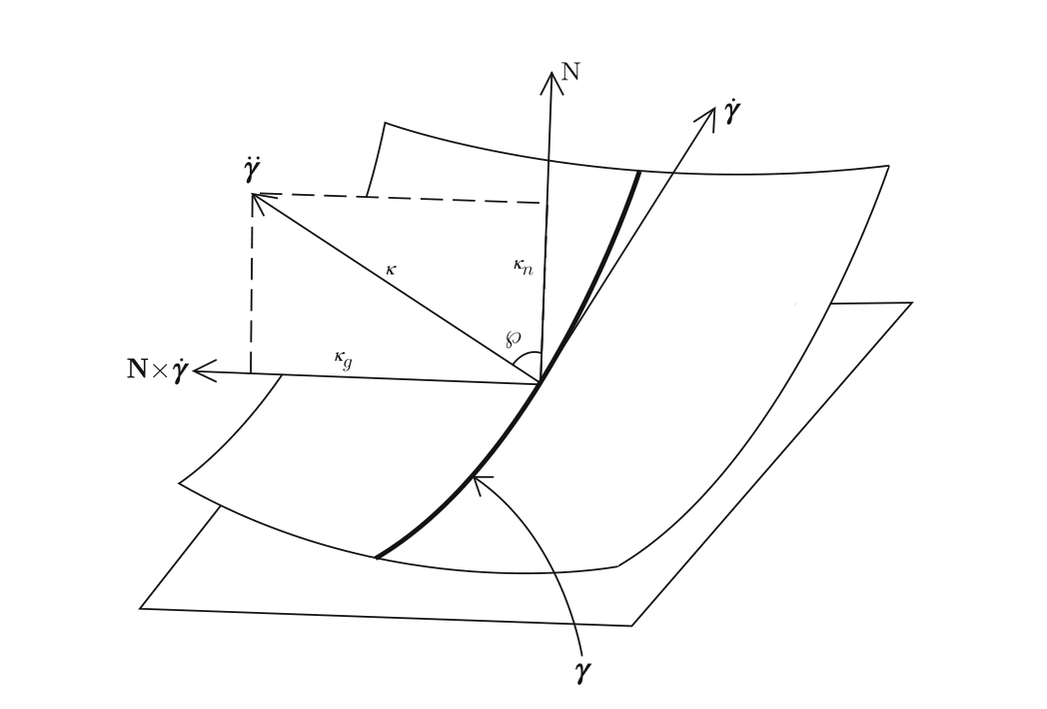
\includegraphics[width=0.65\linewidth]{figures/dgeo_4.1.png}
\end{figure}
\begin{definition}[]
    The scalars $\kappa_n $ and $\kappa_g$ are the \textbf{normal curvature} and \textbf{geodesic curvature} of $\gamma $, respectively.
\end{definition}
Note that these change sign when $\mathbf N$ does, so in general only the magnitudes of $\kappa_n $ and $\kappa_s$ are well defined.

\begin{prop}
    We have 
    \begin{align*}
        \kappa_n &=\ddot \gamma \cdot \mathbf N,\quad \kappa_g = \ddot \gamma \cdot (\mathbf N\times \dot \gamma ),\\
        \kappa^2&=\kappa_n ^2+\kappa_g^2,\\
        \kappa_n &=\kappa \cos \psi, \quad \kappa_g =\pm \kappa\sin \psi,
    \end{align*}
    where $\kappa$ is the curvature of $\gamma $ and $\psi$ is the angle between $\mathbf N$ and the principal normal $\mathbf n$ of $\gamma $.
\end{prop}
\begin{proof}
    To show $\kappa_n =\ddot \gamma \cdot \mathbf N$, note that $\ddot \gamma =\kappa_n \mathbf N+\kappa_g(\mathbf N\times \dot \gamma )$, so $\ddot \gamma \cdot \mathbf N=\kappa_n \mathbf N\cdot \mathbf N+\kappa_g (\mathbf N\times \dot \gamma )\cdot \mathbf N$, which implies that $\ddot \gamma \cdot \mathbf N=\kappa_n $ since the vectors $\mathbf N$ and $\mathbf N\times \dot\gamma $ are orthogonal. A similar process shows that $\kappa_g=\ddot \gamma \cdot (\mathbf N\times \dot \gamma )$. {\color{red}todo:not sure how to show $\kappa^2=\kappa_n ^2+\kappa_g^2$?} Since $\ddot \gamma =\kappa n$, {\color{red}todo:?} 
\end{proof}
As a unit speed parameter $t$ is changed to another parameter $\pm t+c$, then $\kappa_n \mapsto \kappa_n $ and $\kappa_g \mapsto  \pm \kappa_g$, so $\kappa_n $ is well defined for any regular curve while $\kappa_g$ is only well defined up to sign.

\begin{prop}
    If $\gamma $ is unit-speed on an oriented surface $S,$ its normal curvature is given by $\kappa_n =\langle \langle \dot \gamma ,\dot \gamma  \rangle  \rangle $. If $\sigma$ is a surface patch of $S$ and $\gamma (t)=\sigma(u(t),v(t))$ is a curve in $\sigma$, then we also have $\kappa_n =L\dot u^2+2M\dot u \dot v+N\dot v^2$.
\end{prop}
So two curves that interset at $p$ and have the parallel tangent vectors there have the same normal curvature at $p$. {\color{red}todo:how?} 
\begin{proof}
    Since $\dot \gamma $ is tangent to $S$, $\mathbf N \cdot \dot \gamma =0$. So $\mathbf N\cdot \ddot \gamma =-\dot{\mathbf N} \cdot \dot \gamma $. Note that $\dot{\mathbf N} = \frac{d}{dt}\mathcal{G} (\gamma (t))=-\mathcal{W} (\dot \gamma )$, therefore\[
        \kappa_n =\mathbf N\cdot \ddot \gamma =-\dot{\mathbf N} \cdot \dot \gamma =\langle \mathcal{W} (\dot \gamma ),\dot \gamma  \rangle =\langle \langle \dot \gamma ,\dot \gamma  \rangle  \rangle .\qedhere
    \] 
\end{proof}
While the normal curvature depends on the sff, the geodesic curvature only depends on the fff. 
\begin{namedthm}{Meusnier's Theorem} 
   Let $p \in S$ and $v \in T_p S$. Let $\Pi _{\theta}$ be the plane spanned by $v$ and making an angle $\theta$ with $T_p S$. Suppose $\Pi_{\theta}$ intersects $S$ at a curve with curvature $\kappa_{\theta}$. Then $\kappa_{\theta}\sin \theta$ is independent of $\theta$.
\begin{figure}[H]
\centering
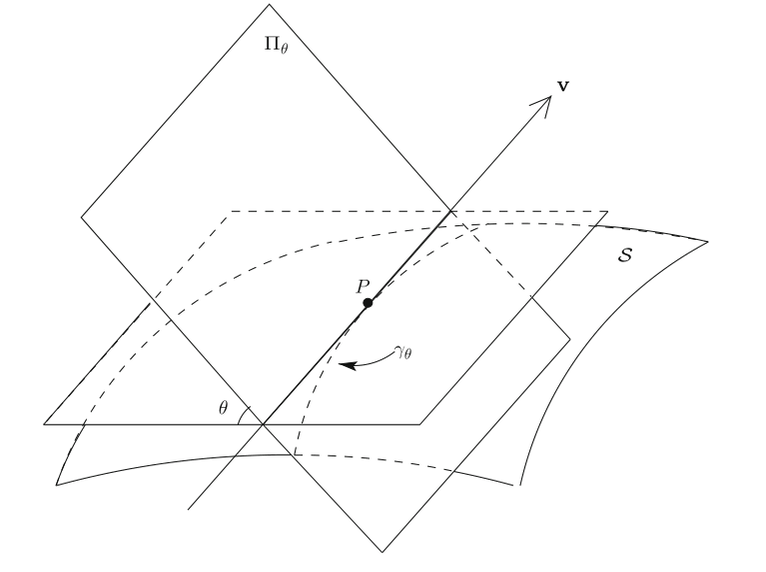
\includegraphics[width=0.6\linewidth]{figures/dgeo_4.2.png}
\end{figure}
\end{namedthm}
\begin{proof}
    Suppose $\gamma _{\theta}$ is a unit speed parametrization of the aforementioned curve. Then at $p, \dot \gamma _{\theta}=\pm v$, so $\ddot \gamma _{\theta}$ is perpendicular to $v$ and parallel to $\Pi_{\theta}$. Then $\psi = \pi /2 -\theta$, so $\kappa_n =\kappa_{\theta}\cos(\pi /2-\theta)=\kappa_{\theta}\sin \theta$, but $\kappa_n $ does not depend on $\theta$.
\end{proof}
An important case is where $\gamma $ is a \textbf{normal section} of the surface, i.e., $\gamma $ is the intersection of the surface with a plane $\Pi$ that is orthogonal to the tangent plane of the surface at each point of $\gamma $.

\begin{cor}
    The curvature, normal curvature $\kappa_n $, and geodesic curvature $\kappa_g$ of a normal section of a surface are related by $\kappa_n =\pm \kappa,\ \kappa_g=0$.
\end{cor}
\begin{proof}
    We have $\kappa_n =\kappa\sin \theta$ where $\theta=\pm\pi /2$. For the second part, $\kappa^2=\kappa_n ^2+\kappa_g^2$, and since $\kappa=\pm \kappa_n ,$ we must have $\kappa_g=0$.
\end{proof}

\subsection{Parallel transport and the covariant derivative}

